%%%%%%%%%%%%%%%%%%%%%%%%%%%%%%%%%%%%%%%%%%%%%%%%%%%%%%%%%%%%%%%%%%%%%%%%%%%
%% This file is part of the book
%%
%% Algorithmic Graph Theory
%% http://code.google.com/p/graph-theory-algorithms-book/
%%
%% Copyright (C) 2009, 2010, 2011 Minh Van Nguyen <nguyenminh2@gmail.com>
%%
%% See the file COPYING for copying conditions.
%%%%%%%%%%%%%%%%%%%%%%%%%%%%%%%%%%%%%%%%%%%%%%%%%%%%%%%%%%%%%%%%%%%%%%%%%%%

%% wheel graph W_6
\subfigure[$G_1$]{
\label{fig:introduction:contracting_wheel_graph_W6}
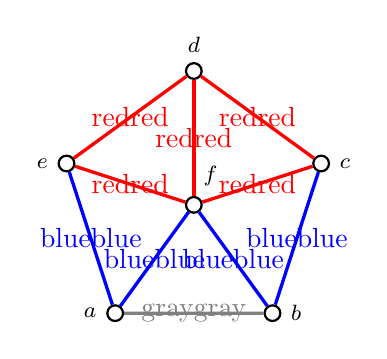
\begin{tikzpicture}
[lineDecorate/.style={-,very thick},%
  nodeDecorate/.style={shape=circle,inner sep=2pt,draw,thick},%
  scale=1.7]
%% nodes or vertices
\foreach \nodename/\x/\y/\direction/\navigate in {
  a/-0.5877/-0.8090/left/west, b/0.5877/-0.8090/right/east,
  c/0.9510/0.3090/right/east, d/0/1/above/north,
  e/-0.9510/0.3090/left/west, f/0/0/above right/north}
{
  \node (\nodename) at (\x,\y) [nodeDecorate] {};
  \node [\direction] at (\nodename.\navigate) {\footnotesize$\nodename$};
}
%% edges or lines
\path
\foreach \startnode/\endnode/\color in {
  c/d/red, c/b/blue, c/f/red, d/e/red, d/f/red, e/a/blue, e/f/red,
  a/b/gray, a/f/blue, b/f/blue}
{
  (\startnode) edge[lineDecorate,color=\color] node {} (\endnode)
};
\end{tikzpicture}
}
%%
%%
%% edge contraction W_6/ab
\subfigure[$G_2 = G_1/ab$]{
\label{fig:introduction:contracting_wheel_graph_W5}
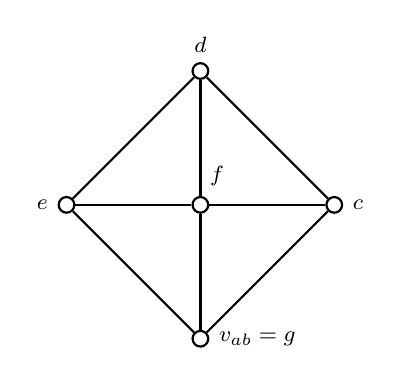
\begin{tikzpicture}
[lineDecorate/.style={-,thick},%
  nodeDecorate/.style={shape=circle,inner sep=2pt,draw,thick},%
  scale=1.7]
%% nodes or vertices
\foreach \nodename/\x/\y/\direction/\navigate in {
  c/1/0/right/east, d/0/1/above/north, e/-1/0/left/west,
  f/0/0/above right/north}
{
  \node (\nodename) at (\x,\y) [nodeDecorate] {};
  \node [\direction] at (\nodename.\navigate) {\footnotesize$\nodename$};
}
\node (ab) at (0,-1) [nodeDecorate] {};
\node [right] at (ab.east) {\footnotesize$v_{ab} = g$};
%% edges or lines
\path
\foreach \startnode/\endnode in {
  c/d, c/ab, c/f, d/e, d/f, e/ab, e/f, ab/f}
{
  (\startnode) edge[lineDecorate] node {} (\endnode)
};
\end{tikzpicture}
}
%%
%%
%% edge contraction G_2/cg
\subfigure[$G_3 = G_2/cg$]{
\label{fig:introduction:contracting_wheel_graph_W4}
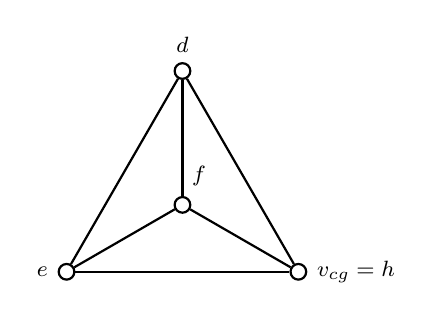
\begin{tikzpicture}
[lineDecorate/.style={-,thick},%
  nodeDecorate/.style={shape=circle,inner sep=2pt,draw,thick},%
  scale=1.7]
%% nodes or vertices
\foreach \nodename/\x/\y/\direction/\navigate in {
  d/0/1/above/north, e/-0.8660/-0.5/left/west, f/0/0/above right/north}
{
  \node (\nodename) at (\x,\y) [nodeDecorate] {};
  \node [\direction] at (\nodename.\navigate) {\footnotesize$\nodename$};
}
\node (cg) at (0.8660,-0.5) [nodeDecorate] {};
\node [right] at (cg.east) {\footnotesize$v_{cg} = h$};
%% edges or lines
\path
\foreach \startnode/\endnode in {cg/d, cg/e, cg/f, d/e, d/f, e/f}
{
  (\startnode) edge[lineDecorate] node {} (\endnode)
};
\end{tikzpicture}
}
%%
%%
%% edge contraction G_3/dh
\subfigure[$G_4 = G_3/dh$]{
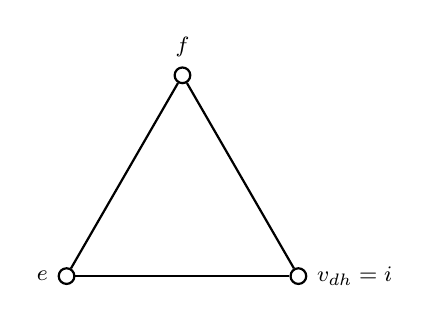
\begin{tikzpicture}
[lineDecorate/.style={-,thick},%
  nodeDecorate/.style={shape=circle,inner sep=2pt,draw,thick},%
  scale=1.7]
%% nodes or vertices
\foreach \nodename/\x/\y/\direction/\navigate in {
  f/0/1/above/north, e/-0.8660/-0.5/left/west}
{
  \node (\nodename) at (\x,\y) [nodeDecorate] {};
  \node [\direction] at (\nodename.\navigate) {\footnotesize$\nodename$};
}
\node (dh) at (0.8660,-0.5) [nodeDecorate] {};
\node [right] at (dh.east) {\footnotesize$v_{dh} = i$};
%% edges or lines
\path
\foreach \startnode/\endnode in {dh/f, dh/e, e/f}
{
  (\startnode) edge[lineDecorate] node {} (\endnode)
};
\end{tikzpicture}
}
%%
%%
%% edge contraction G_4/fi
\subfigure[$G_5 = G_4/fi$]{
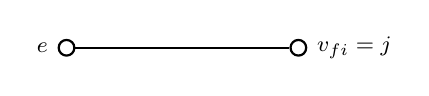
\begin{tikzpicture}
[lineDecorate/.style={-,thick},%
  nodeDecorate/.style={shape=circle,inner sep=2pt,draw,thick},%
  scale=1.7]
%% nodes or vertices
\node (e) at (-0.8660,-0.5) [nodeDecorate] {};
\node [left] at (e.west) {\footnotesize$e$};
\node (fi) at (0.8660,-0.5) [nodeDecorate] {};
\node [right] at (fi.east) {\footnotesize$v_{fi} = j$};
%% edges or lines
\path (e) edge[lineDecorate] node {} (fi);
\end{tikzpicture}
}
%%
%%
%% edge contraction G_5/ej
\subfigure[$G_6 = G_5/ej$]{
\label{fig:introduction:wheel_graph_W6_contracted_to_K1}
\begin{tikzpicture}
[lineDecorate/.style={-,thick},%
  nodeDecorate/.style={shape=circle,inner sep=2pt,draw,thick},%
  scale=1.7]
%% nodes or vertices
\node (ej) at (0,0) [nodeDecorate] {};
\node [right] at (ej.east) {\footnotesize$v_{ej}$};
%% stub node that should not be visible
\node (stub1) at (1,0) [] {};
\node (stub2) at (-1,0) [] {};
\end{tikzpicture}
}
